\newpage
\section{Projekt-  und Analyseergebnisse}
\label{projekt_und_analyseergebnisse}

Im folgenden Kapitel werden die Analyseergebnisse beschrieben, die innerhalb der Arbeitspakete 1~bis~3 erzielt worden sind. Da die Ergebnisse inhaltlich aufeinander aufbauen, werden sie, beginnend mit dem Arbeitspaket~1, entlang der Arbeitspakete beschrieben.

\subsection{Arbeitspaket 1: Beschreibung der Ist-Situation}
\label{arbeitspaket_1_beschreibung_der_ist_situation}

\subsubsection{Betrachtung der Verteilung von Wohngebieten und der Einwohnerdichte}

Durch die Betrachtung der Verteilung von Wohngebieten in Verbindung mit der Einwohnerdichte ermöglicht es im weiteren Verlauf Rückschlüsse auf besonders wichtige Teile der Verkehrsinfrastruktur zu ziehen. Besonders große und dicht besiedelte Wohngebiete sind auf eine entsprechend dimensionierte Verkehrsinfrastruktur angewiesen.

Die bewohnte Fläche im Berliner Stadtgebiet beläuft sich auf ungefähr 368 Quadratkilometer. Das bedeutet, dass ca. 41~\% der gesamten Berliner Landfläche (892~Quadratkilometer) durch Wohngebiete beansprucht wird. Bei der Betrachtung der Berliner Wohngebiete ist auffällig, dass die Flächen im Osten der Stadt deutlich großzügiger geschnitten sind als die Wohngebiete in den zentralen Bezirken und im Westen der Stadt. Grundsätzlich lässt sich aber erkennen, dass die Wohngebiete nahezu gleichmäßig über das Berliner Stadtgebiet verteilt sind.

Durch die zusätzliche Betrachtung der Einwohnerdichte können Rückschlüsse auf die tatsächliche Verteilung der Anzahl von Bürger*innen im Stadtgebiet gezogen werden. Bis auf einzelne Ausnahmen zeigt sich, dass die zentralen Bezirke der Stadt deutlich dichter besiedelt sind als die Außenbezirke.

Die Flächen mit der höchsten Bevölkerungsdichte befinden sich in

\begin{itemize}
    \item 10623 Charlottenburg
    \item 12107 Mariendorf im Ortsteil Tempelhof-Schöneberg
    \item 12623 Kaulsdorf-Mahlsdorf
\end{itemize}

\img{karte-einwohnerdichte}{karte-einwohnerdichte}{width=14cm}{Verteilung der Einwohnerdichte und die 3 Flächen mit der höchsten Bevölkerungsdichte: Mariendorf, Tempelhof und Kaulsdorf-Mahlsdorf}

Die Wohngebiete in den Außenbezirken weisen im Vergleich zu den zentralen Bezirken zwar eine deutlich geringere Einwohnerdichte auf, machen aber aufgrund der größeren Fläche einen beträchtlichen Anteil der Einwohnerzahlen aus. Diese Dezentralität stellt eine Herausforderung für die Berliner Verkehrsinfrastruktur dar. Anders als in stark zentralisierten Städten, gilt es in Berlin die Anbindung vieler Kieze in einem großen Stadtgebiet auch untereinander sicherzustellen.

\subsubsection{Arbeitsplätze, Bildungseinrichtungen und Einkaufsmöglichkeiten als Eckpunkte der urbanen Mobilität}

Neben den dicht besiedelten Wohngebieten stellen Pendlerziele wie Arbeitsstätten, Bildungseinrichtungen und Einkaufsmöglichkeiten weitere Eckpfeiler der urbanen Mobilität dar. Die Analyse der relevanten Geodaten zeigt, dass Handels- und Dienstleistungszentren sowie die Universitäten fast gleichmäßig über das Stadtgebiet verteilt sind. Nur wenige Bereiche, wie der Bezirk Steglitz-Zehlendorf im Südwesten der Stadt sowie die Bezirke Treptow-Köpenick und der Ortsteil Rudow im Bezirk Neukölln weisen ein verhältnismäßig geringes Handels- und Dienstleistungsangebot auf. In den zentralen Bezirken findet sich wiederum ein etwas dichteres Handels- und Dienstleistungsangebot.

Anders verhält es sich bei der Verteilung dedizierter Gewerbe- und Industriegebiete. Große Industriegebiete wie Siemensstadt und der ECONOPARK, befinden sich eher in den Außenbezirken. Am Beispiel des Standorts Adlershofs wird zudem deutlich, dass Gewerbegebiete häufig in unmittelbarer Nähe zu Bildungseinrichtungen gelegen sind. Diese Gewerbe- und Wissenschaftsstandorte sind ebenfalls in den äußeren Gebieten der Stadt angesiedelt. Gleiches gilt für Gebiete, die Handel, Dienstleistungen und Industrie als Gewerbe- und Industriepark bündeln.

\img{karte-arbeitsplaetze}{karte-arbeitsplaetze}{width=14cm}{Verteilung der Arbeitsplätze, Bildungseinrichtungen und Einkaufsmöglichkeiten}

\subsubsection{Das Berliner Straßennetz}

Die oben beschriebenen Orte bilden die Eckpunkte der Berliner Mobilität. Diese stark frequentierten Orte, sind durch eine vielschichtige Verkehrsinfrastruktur miteinander vernetzt. Die einzelnen Ebenen dieser Infrastruktur werden im Folgenden auf Basis der vorliegenden Geodaten beschrieben. Diese Beschreibung der Ist-Situation ist Ausgangspunkt für die Identifizierung von Schwachstellen innerhalb der vorhandenen Infrastruktur, die in Arbeitspaket 2 vorgenommen wird.

Das Straßennetz bildet eines der zentralen Elemente dieser Infrastruktur. Insgesamt stehen den Berliner Bürger*innen 5.437~Kilometer öffentlicher Straßen zur Verfügung. Diese nehmen ca. 11~\% der Gesamtfläche der Stadt in Anspruch. Auf ungefähr 80~\% des gesamten Straßennetzes gilt ein Tempolimit von 30~km/h. Die restlichen Straßen teilen sich in 15~\% innerstädtische Hauptverkehrsstraßen mit einer Geschwindigkeitsbegrenzung von 50~km/h und 5~\% restliche Straßen, die sich aus 60er-Zonen, 80er-Zonen, verkehrsberuhigten Bereichen, der Stadtautobahn und anderen begrenzt befahrbaren Flächen zusammensetzen. Ein Blick auf die Verteilung der Tempolimits zeigt, dass ein Großteil der 30er-Zonen in Wohngebieten sowie um Schulen und Kindertagesstätten zu finden ist. Die verkehrsberuhigten Bereiche sind meist durch Straßen mit einer zulässigen Höchstgeschwindigkeit von~50 km/h verbunden.

\img{karte-strassen}{karte-strassen}{width=14cm}{Verteilung der zulässigen Höchstgeschwindigkeiten im Berliner Straßennetz}

Anhand eines Vergleichs der tatsächlich gefahrenen Geschwindigkeiten und der zulässigen Höchstgeschwindigkeiten wird deutlich, dass sich der Straßenverkehr meist langsamer fortbewegt als erlaubt.

\img{tatsaechlich-speed}{tatsaechlich-speed}{width=14cm}{Verteilung der tatsächlich gefahrenen Höchstgeschwindigkeiten im Tagesverlauf an Wochentagen}

Während der morgendlichen und abendlichen Stoßzeiten an Wochentagen, beträgt die Durchschnittsgeschwindigkeit teilweise weniger als 50~\% der zulässigen Maximalgeschwindigkeit. Die niedrigste Durchschnittsgeschwindigkeit findet sich in den Nachmittags- und Abendstunden. Daraus folgt, dass das Berliner Straßennetz zu den Hauptverkehrszeiten an die Kapazitätsgrenzen stößt und, dass der ÖPNV für viele Verkehrsteilnehmer*innen keine adäquate Alternative darstellt.

\subsubsection{Der Bestand dedizierter Radverkehrsanlagen}

Aktuell existieren insgesamt 1.533~Kilometer dedizierter Radverkehrsanlagen – also Radspuren, Radwege oder Busspuren, die von Radfahrern genutzt werden und für diese ausgewiesen sind. In der Stadtmitte gibt es verhältnismäßig viele Radanlagen. In den Außenbezirken und auf kleineren Straßen teilt sich der motorisierte Verkehr und der Fahrradverkehr jedoch häufig die gleiche Fahrspur. Der Großteil der vorhandenen Fahrradwege verläuft aktuell auf Bürgersteigen neben den Gehwegen (1.238~Kilometer).

\img{karte-radnetz}{karte-radnetz}{width=14cm}{Verteilung dedizierter Radverkehrsanlagen im Berliner Straßennetz; eingefärbt nach Länge des Segments}

Die Betrachtung der Radverkehrsanlagen zeigt zudem, dass zahlreiche Unterbrechungen auf den Fahrradwegen existieren. Die durchschnittliche Länge einer Fahrradspur ohne Unterbrechung misst lediglich 81 Meter zwischen zwei Kreuzungen. Die längste Fahrradspur ohne Unterbrechung erstreckt sich über 1,73~Kilometer.

\subsubsection{Die Berliner ÖPNV-Infrastruktur}

Die Berliner ÖPNV-Infrastruktur umfasst U-Bahnen, Straßenbahnen, S-Bahnen und Busse. Die Gesamtstrecke des ÖPNV beläuft sich auf 2.600~Kilometer Länge.

\img{karte-oepnv}{karte-oepnv}{width=14cm}{Übersicht des Berliner ÖPNV-Netzes bestehend aus U-Bahnen, Straßenbahnen, S-Bahnen und Bussen}

Allein die U-Bahninfrastruktur besteht aus 10 Linien die mit über 1.200~Wagen die 173~U-Bahnhöfe im Stadtgebiet bedienen. Die U-Bahnlinien konzentrieren sich vor allem auf die zentralen Bezirke. Dies sorgt in den zentralen Bezirken für eine hohe Flexibilität durch viele Umsteigemöglichkeiten. Die Außenbezirke werden in der Regel nur von einzelnen Linien bedient.

In den östlichen Bezirken der Stadt verkehren täglich 22~Straßenbahnlinien mit 342~Fahrzeugen auf einem engmaschigen Netz mit 803~Haltestellen. Im übrigen Stadtgebiet gibt es aktuell keine direkte Anbindung an das Straßenbahnnetz.

Die Businfrastruktur bietet hingegen eine flächendeckende Anbindung an das ÖPNV-Netz im gesamten Stadtgebiet. Die 6.481 Bushaltestellen stehen nahezu gleichmäßig über die gesamte Fläche der Stadt verteilt zur Verfügung. Ausgehend von den 154~Buslinien bildet die Businfrastruktur ein dichtes und weitreichendes Verkehrsnetz.

Die Infrastruktur der BVG wird durch 16~S-Bahnlinien ergänzt, die 166 S-Bahnhöfe bedienen und durch die VBB betrieben werden. Für die S-Bahnen stehen in Berlin und dem direkten Stadtumfeld (Tarifbereich C) Schieneninfrastruktur auf einer Länge von 335~Kilometern zur Verfügung.

\subsection{Arbeitspaket 2: Aufzeigen von Schwachstellen der vorhandenen Verkehrsinfrastruktur}
\label{arbeitspaket_2_aufzeigen_von_schwachstellen_der_vorhandenen_infrastruktur}

Die Identifizierung von Schwachstellen in der vorhandenen Verkehrsinfrastruktur, basiert auf der Berechnung der 15-Minuten-Isochrone für 10.000 randomisiert ausgewählte Orte in Berlin. Ausgehend von diesen Orten wird die Anbindungsqualität im Stadtbild berechnet und mithilfe einer Farbkodierung sichtbar gemacht (für eine detailierte Beschreibung der Methodik, siehe Kapitel~\ref{projektumsetzung}). Die Berechnung der Anbindungsqualität ist Voraussetzung dafür, dass einzelne Gebiete für die Entwicklung von Lösungsansätzen priorisiert werden können (siehe Kapitel~\ref{arbeitspaket_3_ableiten_von_handlungsempfehlungen}).

\subsubsection{Motorisierter Individualverkehr}

Die Erreichbarkeit durch den motorisierten Individualverkehr ist in Berlin weitgehend gegeben. Die Analyse der tatsächlichen Geschwindigkeit des motorisierten Individualverkehrs zeigt deutlich, dass die Straßeninfrastruktur in weiten Teilen der Stadt eine hohe Erreichbarkeit gewährleistet. Auf der Stadtautobahn legen Bürger*innen bis zu 27~Kilometer in 15~Minuten zurück. Das stellt unter den betrachteten Verkehrsmitteln den höchstwert dar.

\img{erreichbarkeit-miv}{erreichbarkeit-miv}{width=14cm}{Abbildung der innerstädtischen 15-Minuten-Isochrone bei Nutzung des motorisierten Individualverkehrs}

Ein direkter geografischer Vergleich innerhalb des Stadtgebiets zeigt, dass die Bereiche südwestlich vom Stadtzentrum stark von der Nähe zur Stadtautobahn A100 profitieren. Bezirke wie Tempelhof-Schöneberg und Charlottenburg-Wilmersdorf weisen eine deutlich höhere Erreichbarkeit auf, als die Bezirke im Osten der Stadt. Ausgehend vom Stadtteil Charlottenburg legen Autofahrer*innen durchschnittlich 15,5~Kilometer in 15~Minuten zurück.

Weniger gut angebundene Gebiete finden sich auch an den Stadträndern. Bei Kladow im Südwesten der Stadt wird die Erreichbarkeit durch den Verlauf der Havel erschwert. Auch im Norden der Stadt gibt es um den Ortsteil Französisch Buchholz Gebiete, die mit dem Auto weniger gut zu erreichen sind.

\subsubsection{Fahrradverkehr}

Für den Vergleich der Erreichbarkeit mit dem Fahrrad wird ausschließlich die Nutzung der ausgewiesenen Radinfrastruktur betrachtet. Da viele Berliner*innen es aufgrund von Sicherheitsbedenken vermeiden, Hauptverkehrsstraßen ohne Fahrradweg zu befahren, wurden diese explizit von der Analyse ausgeschlossen. Das Resultat zeigt deutlich, dass Gebiete in den zentralen Bezirken im Vergleich zu den Orten in den Außenbezirken über eine verhältnismäßig gut ausgebaute Radinfrastruktur verfügen.

\img{erreichbarkeit-bike}{erreichbarkeit-bike}{width=14cm}{Abbildung der innerstädtischen 15-Minuten-Isochrone für den Fahrradverkehr}

Ausgehend von den zentralen Bezirken legt eine Fahrradfahrerin innerhalb von 15 Minuten eine Distanz von bis zu 3,8~Kilometern zurück und erreicht damit eine Durchschnittsgeschwindigkeit von circa 15,2~km/h. Im Vergleich zu führenden internationalen Fahrradstädten wie Kopenhagen wird deutlich, dass es hier noch großes Steigerungspotenzial gibt. In Kopenhagen beträgt die durchschnittliche Geschwindigkeit des Fahrradverkehrs 16,3~km/h.\footcite{kopenhagen}
Diese Geschwindigkeit wird selbst in den besser angebundenen Gebieten der Berliner Innenstadt nicht erreicht. Die Fahrradanbindung nimmt in Richtung des Stadtrands zudem rapide ab. Lediglich die nord-westlichen Bezirke stellen hier eine Ausnahme dar. Die berechnete Erreichbarkeit einzelner Orte im Stadtgebiet, bestätigt demnach die Lücken in der Fahrradinfrastruktur, die bereits in den Ergebnissen zu Arbeitspaket 1 angedeutet werden.

\subsubsection{Businfrastruktur}

Während Bürger*innen mit dem Auto in 15~Minuten bis zu 27~Kilometer zurücklegen können, beträgt die maximal erreichbare Distanz mit dem Bus lediglich 4,7~Kilometer. Da es hinsichtlich der Erreichbarkeit von Bushaltestellen im Stadtgebiet keine signifikanten Unterschiede gibt, bietet der Bus im Vergleich mit anderen Verkehrsmitteln eine konstante, aber in Bezug auf die zurücklegbare Distanz stark limitierte Anbindung. Im Durchschnitt lässt sich mit dem Bus innerhalb von 15~Minuten lediglich eine Distanz von ca. 2,9~Kilometer zurücklegen. In der Praxis reduzieren die Taktung und die dadurch entstehenden Wartezeiten die zurückzulegende Distanz zusätzlich. Aus Gründen der Datenverfügbarkeit und der Komplexität wurden  Umstiegs- und Wartezeiten allerdings in der vorliegenden Analyse für alle Verkehrsmittel außer acht gelassen. Dieser Punkt wird im Kapitel~\ref{limitierung} genauer erläutert.

\img{erreichbarkeit-bus}{erreichbarkeit-bus}{width=14cm}{Abbildung der innerstädtischen 15-Minuten-Isochrone für den Busverkehr}

Die Analyse zeigt auch, dass die Anbindungsqualität in Richtung der Außenbezirke leicht abnimmt. Das kann insbesondere durch fehlende Umsteigemöglichkeiten erklärt werden. Weite Teile der Außenbezirke werden durch einzelne Linien bedient, was sich negativ auf die Flexibilität und Erreichbarkeit auswirkt. Wenn weder Bus, Straßenbahn noch U-Bahn oder S-Bahn eine zuverlässige Anbindung an den ÖPNV bieten, ist der Individualverkehr häufig die einzige verbleibende Option für Anwohner*innen in den Außenbzirken.

\subsubsection{S-Bahn-Netz}

Die Analyse der Anbindungsqualität mit der S-Bahn zeigt, dass es ein starkes Gefälle zwischen gut und weniger gut angebundenen Orten innerhalb der Stadt gibt. Insbesondere die innerstädtischen Gebiete profitieren von der Überschneidung mehrerer S-Bahnlinien. So sorgt im Ortsteil Gesundbrunnen der Zugang zu den S-Bahnlinien S1, S2, S25, S41, S42 für eine sehr gute Anbindung. Gleiches gilt für den S-Bahnhof Friedrichstraße mit Zugang zu den Linien S1, S2, S25, S3, S5 und S7 sowie das Gebiet um den Bahnhof Ostkreuz mit direktem Zugang zu den Linien S3, S5, S75, S41 und S42. Ausgehend von diesen Orten können innerhalb von 15 Minuten bis zu 8 Kilometer mit der S-Bahn zurückgelegt werden.

\img{erreichbarkeit-sbahn}{erreichbarkeit-sbahn}{width=14cm}{Abbildung der innerstädtischen 15-Minuten-Isochrone für den S-Bahnverkehr}

Im Gegensatz zu den gut angebundenen Gebieten können Bürger*innen im Süden des Bezirks Neukölln auf keinerlei S-Bahninfrastruktur zurückgreifen. Insbesondere die Ortsteile Buckow und Rudow sind von der fehlenden S-Bahnanbindung betroffen. Selbst in weiten Teilen des an den S-Bahn-Ring grenzenden Britz, ist keine S-Bahnstation fußläufig (d. h. innerhalb von 15~Minuten) zu erreichen. Gleiches gilt für den Ortsteil Charlottenburg-Nord sowie den Ortsteil Weißensee.

\subsubsection{U-Bahn-Netz}

Im Gegensatz zur S-Bahn existiert hinsichtlich der U-Bahninfrastruktur, ein deutlich geringeres Gefälle zwischen den gut und den weniger gut angebundenen Gebieten. Die Berechnung der Anbindungsqualität zeigt, dass die U-Bahn in den zentralen Bezirken eine verlässliche Anbindung sicherstellt. Dabei sorgt beispielsweise die Linie U1 für eine hohe Interkonnektivität mit anderen U-Bahnlinien in den Bezirken Friedrichshain-Kreuzberg und Charlottenburg-Wilmersdorf. In diesen zentralen Bezirken lassen sich mit der U-Bahn innerhalb von 15~Minuten bis zu 7,2~Kilometer zurücklegen.

\img{erreichbarkeit-ubahn}{erreichbarkeit-ubahn}{width=14cm}{Abbildung der innerstädtischen 15-Minuten-Isochrone für den U-Bahnverkehr}

Das Stadtgebiet jenseits der zentralen Bezirke ist lediglich über einzelne Linien an das U-Bahnnetz angebunden. Die Linie U3 bindet beispielsweise den Bezirk Steglitz-Zehlendorf an das U-Bahnnetz an, bietet jedoch erst an der zehnten Station die Möglichkeit zum Umstieg auf eine andere U-Bahnlinie. Eine ähnliche Situation zeigt sich auch in Hönow und Weißensee im Osten des Bezirks Pankow. Im Durchschnitt können hier 5,6 km innerhalb von 15~Minuten zurückgelegt werden. In anderen Gebieten, insbesondere in den Außenbezirken, befindet sich keine U-Bahnstation in Laufentfernung.

\subsubsection{Gesamtes ÖPNV-Netz}

Die isolierte Betrachtung der Verkehrsmittel ermöglicht Einblicke in die Herausforderungen auf den einzelnen Ebenen der Verkehrsinfrastruktur. Diese isolierte Betrachtung ist jedoch nur bedingt hilfreich, um übergreifende Herausforderungen zu identifizieren. Ziel des folgenden Abschnitts ist es, ein besseres Verständnis für die Probleme der Verkehrsinfrastruktur zu schaffen, die im Fokus der Verkehrswende gezielt ausgebaut werden soll. Demnach wird der ÖPNV – also S-Bahnen, U-Bahnen, Busse und Straßenbahnen – betrachtet. Da der Autoverkehr nicht im Fokus der Verkehrswende steht, wird die Auto-Infrastruktur an dieser Stelle nicht weiter berücksichtigt.

Für diese verkehrsmittelübergreifende Analyse werden die Daten aller relevanten Verkehrsmittel miteinander verknüpft. Dadurch können bei der Berechnung der Anbindungsqualität Umstiege und Wechsel zwischen Verkehrsmitteln berücksichtigt werden. Das Bedeutet, dass durch die verkehrsmittelübergreifenden 15-Minuten-Isochronen alle Wege berechnet werden, von einem gegebenen Ort in 15~Minuten zurückgelegt werden können. Die verkehrsmittelübergreinfenden Isochronen bilden demnach die Grundlage für die datengestützte Identifizierung übergreifender Infrastrukturprobleme.

\img{erreichbarkeit-opnv}{erreichbarkeit-opnv}{width=14cm}{Abbildung der innerstädtischen 15-Minuten-Isochrone aggregiert für den gesamten öffentlichen Personennahverkehr in Berlin}

Die verkehrsmittelübergreifende Analyse der Anbindungsqualität zeigt, dass sich die Orte mit der verhältnismäßig besten Anbindung in den zentralen Bezirken befinden. Insbesondere die Bürger*innen im Ortsteil Gesundbrunnen und im angrenzenden Arnimkiez haben bereits heute Zugang zu einer engmaschigen Verkehrsinfrastruktur. Gleiches gilt für das Gebiet um die Friedrichstraße und das westliche Ende der Torstraße sowie das Gebiet um den Bahnhof Potsdamer Platz. Auch im Südosten der Stadt ist grundsätzlich eine dichte Verkehrsinfrastruktur gegeben. Dabei stechen insbesondere die Gebiete um den Bahnhof Ostkreuz und den Bahnhof Baumschulenweg sowie das Gebiet zwischen den Bahnhöfen Neukölln und Hermannstraße hervor.

Im Gegensatz zu den gut angebundenen Gebieten im Zentrum und Südosten der Stadt finden sich vor allem in den Außenbezirken Gebiete ohne ausreichende Anbindung. Beispielsweise Kladow, der südlichste Ortsteil der Stadt, ist lediglich mit dem Bus erreichbar, sodass die übergreifende Verkehrsanbindung gering ausfällt. Die Anbindungsqualität in den Ortsteilen Müggelheim und Französisch Buchholz ist ebenfalls auf einem sehr geringen Niveau.

Die Analyse zeigt überraschenderweise auch, dass selbst einige der zentralen Gebiete nicht über eine zuverlässige Anbindung an die Verkehrsinfrastruktur verfügen. Weder der Ortsteil Moabit, noch der Gräfekiez in Kreuzberg zeichnen sich durch eine hohe Erreichbarkeit aus. Gleiches gilt für den Ortsteil Alt-Hohenschönhausen und den gesamten Süden der Stadt jenseits des S-Bahnrings.

\subsection{Arbeitspaket 3: Ableiten von Handlungsempfehlungen}
\label{arbeitspaket_3_ableiten_von_handlungsempfehlungen}

Im folgenden Kapitel werden Handlungsempfehlungen für fünf Orte im Berliner Stadtgebiet entwickelt, die zunächst ausgehend von der Analyse der Verkehrsinfrastruktur priorisiert wurden. Die Priorisierung der Orte basiert auf der Betrachtung der Anbindungsqualität und der Relevanz des Ortes für Berliner Bürger*innen. Wichtige Orte mit verhältnismäßig niedriger Anbindungsqualität werden demnach besonders hoch priorisiert. Die Definition wichtiger Orte umfasst, wie in Kapitel~3.1 beschrieben, Handels- und Dienstleistungszentren, Gewerbegebiete sowie Hochschulen und dicht besiedelte Wohngebiete.

Die fünf priorisierten Orte sind über das gesamte Stadtgebiet verteilt. Sie umfassen einen Industriestandort in Spandau, den Zukunftsstandort Urban Tech Republic im ehemaligen Flughafen Tegel, eine Gewerbefläche an der Landsberger Allee, ein dicht besiedeltes Wohngebiet in Marzahn-Hellersdorf sowie ein Gewerbegebiet an der Gradestraße in Britz. Für diese Orte wird zusätzlich zu der quantitativen Analyse (siehe Kapitel ~\ref{arbeitspaket_2_aufzeigen_von_schwachstellen_der_vorhandenen_infrastruktur}), eine qualitative Betrachtung der vorhandenen Infrastruktur sowie laufender und geplanter Infrastrukturprojekte durchgeführt. Auf diese Weise wird ein tiefgreifendes Verständnis für die zugrundeliegenden Problemstellungen etabliert. Ausgehend von den identifizierten Problemen, werden für die priorisierten Orte individuelle Lösungsansätze entwickelt, die zukünftig eine bessere Anbindung ermöglichen könnten.

\subsubsection{Industriestandort Spandau}
\paragraph{Detailbetrachtung der Verkehrsinfrastruktur am Industriestandort Spandau}
Im östlichen Teil Spandaus wird ausgehend von der Betrachtung der Geodaten eine sehr hohe Gewerbedichte festgestellt. Neben dem Ausbildungszentrum der Berliner Polizei befinden sich hier mehrere Möbelhäuser, zwei Kraftwerke, ein Zementwerk und ein Klärwerk. Die Bevölkerungsdichte ist im näheren Umfeld relativ niedrig. Da sich hier jedoch die direkten Pendlerrouten aus dem stark bevölkerten Teil Spandaus und Falkensee schneiden, entsteht ein besonders hohes Pendleraufkommen in beide Verkehrsrichtungen. Laut dem Nahverkehrsplan des Landes Berlin befindet sich hier einer der am meisten ausgelasteten Netzbereiche.

\begin{figure}
    \centering
    \begin{subfigure}{.5\textwidth}
        \centering
        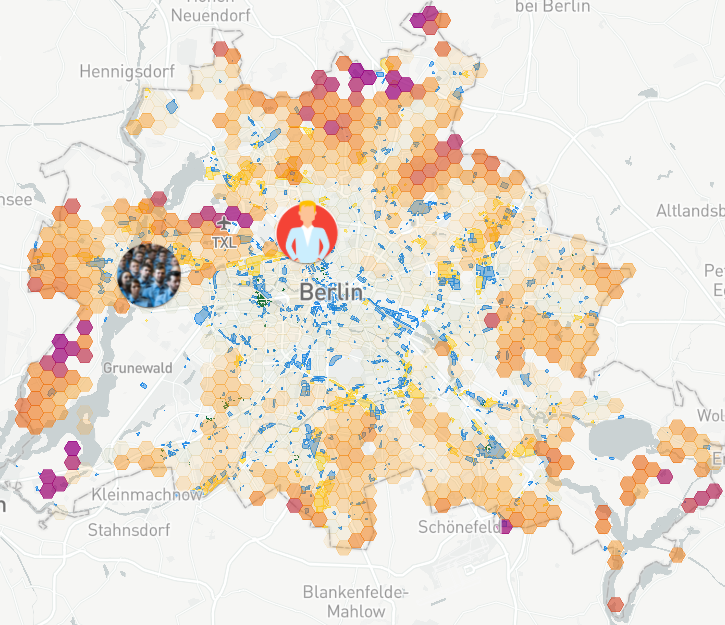
\includegraphics[width=7cm]{persona-spandau-01}
    \end{subfigure}%
    \begin{subfigure}{.5\textwidth}
        \centering
        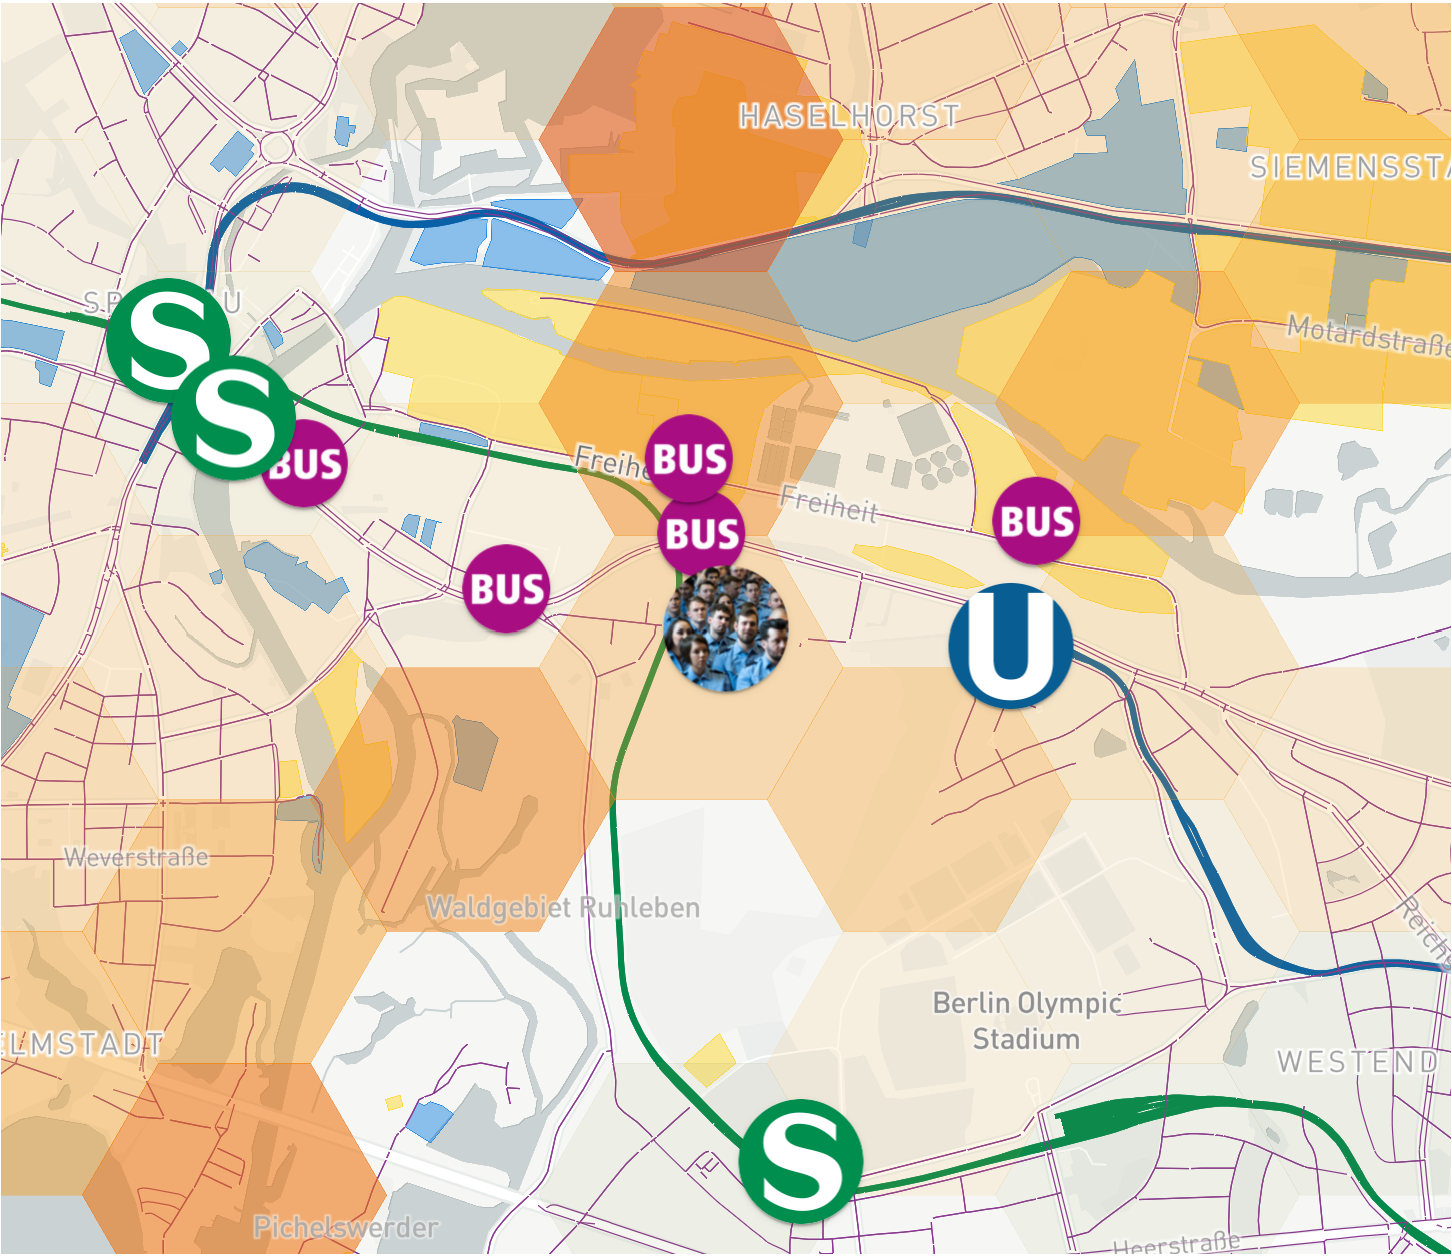
\includegraphics[width=7cm]{persona-spandau-02}
    \end{subfigure}
    \caption{Persona Industriestandort Spandau}
    \label{persona-spandau}
\end{figure}

Für den motorisierten Individualverkehr und den Busverkehr bildet der verlängerte Spandauer Damm die Hauptverkehrsader. Durch das hohe Pendleraufkommen reduziert sich jedoch die Durchschnittsgeschwindigkeit des Verkehrs gerade zu den Stoßzeiten merklich.

Trotz des hohen Verkehrsaufkommens stellen weder U-Bahn noch S-Bahn wegen ihrer großen Entfernung eine praktikable Alternative dar. Die nächste U-Bahnstation (Ruhleben) ist 22~Gehminuten entfernt und bildet mit der U2 eine direkte Verbindung unter anderem zum Zoologischen Garten und zum Alexanderplatz. Die nächste S-Bahnstation (Stresow) befindet sich 33 Gehminuten entfernt und bindet die S-Bahnlinien S9 und S3 sowie den Regionalbahnverkehr an. Fußläufig sind lediglich die Buslinien 131 und M45 erreichbar. Die unterschiedliche Taktung der Bus- und Bahnlinien verhindert jedoch ein schnelles Umsteigen, was sich negativ auf die Attraktivität des Busverkehrs auswirkt.

\paragraph{Lösungsansatz: Verbesserte S-Bahn Anbindung}
Um diesen Umstand zu ändern sieht der Berliner Nahverkehrsplan bereits eine Taktverdichtung des S-Bahnverkehrs auf den Linien S3 und S9 in Spandau vor.\footcite{NahverkehrsplanBerlin} Damit die Bahnverbindungen trotz des weiten Fußwegs als Option für mehr Pendler infrage kommen, sollten Busse eingesetzt werden, um eine direkte Verbindung zu den Bahnstationen herzustellen. Zu den Stoßzeiten sollten diese Busse regelmäßig verkehren, um die Wegzeit der letzten Meile so stark wie möglich zu verkürzen. Außerhalb der Stoßzeiten sollten die Busse als Rufbusse eingesetzt werden, um eine adäquate Anbindung auch während des Schichtbetriebs der angrenzenden Industrie zu gewährleisten.

\subsubsection{Urban Tech Republic - TXL}
\paragraph{Detailbetrachtung der Verkehrsinfrastruktur an der Urban Tech Republic - TXL}
Aufgrund der Mischung aus Wohn- und Gewerbegebiet entsteht in Charlottenburg-Nord viel Pendelverkehr. Nahe dem ehemaligen Flughafen TXL sind große Logistik- und Import-/Export-Unternehmen wie DPD, DB-Schenker und TNT ansässig. Die Einwohnerdichte von Charlottenburg-Nord liegt im Durchschnitt der Stadt.

Trotz geografischer Nähe zur Ringbahn weist dieses Gebiet durch eine geringe Stationsdichte eine schlechte Anbindung an den ÖPNV auf. Lediglich die Buslinie~128 ist fußläufig erreichbar. Um zur nächsten S-Bahnstation (Beusselstraße) zu gelangen, muss ein Fußweg von 28~Minuten zurückgelegt werden. Zur nächsten U-Bahnstation (Jakob-Kaiser-Platz) beträgt der Fußweg sogar 30~Minuten. Die direkte Anbindung an die Stadtautobahn ermöglicht außerhalb der Stoßzeiten eine sehr gute Verbindung mit dem motorisierten Individualverkehr. Auch während des verstärkten Verkehrsaufkommens in den Morgen- und Abendstunden bietet der Individualverkehr die schnellste Verbindung.

\begin{figure}
    \centering
    \begin{subfigure}{.5\textwidth}
        \centering
        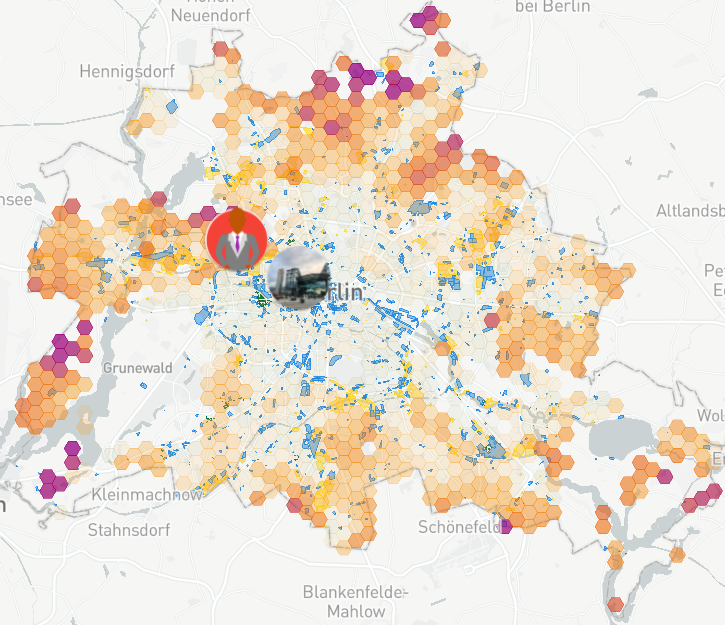
\includegraphics[width=7cm]{persona-charlottenburg-01}
    \end{subfigure}%
    \begin{subfigure}{.5\textwidth}
        \centering
        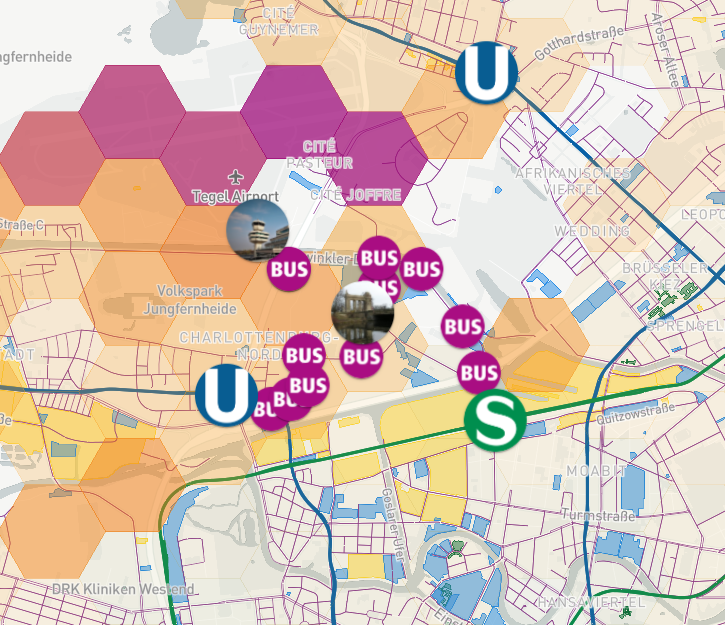
\includegraphics[width=7cm]{persona-charlottenburg-03}
    \end{subfigure}
    \caption{Persona Urban Tech Republic - TXL}
    \label{persona-charlottenburg-nord}
\end{figure}

Als besondere Herausforderung für den Verkehr in Charlottenburg-Nord gilt der Ausbau des ehemaligen Flughafens TXL zum Innovations- und Entwicklungsstandort. Durch die große Anzahl neuer Arbeitsplätze, die hier entstehen sollen, wird prognostiziert, dass das Verkehrsaufkommen merklich steigen wird.\footcite{UrbanTechRepublic} Aufgrund der Begrenzung durch den Berlin-Spandauer-Schifffahrtskanal im Norden und Osten sowie durch den Westhafenkanal im Süden gestaltet sich die Anbindung an die vorhandene Verkehrsinfrastruktur in angrenzenden Gebieten als schwierig.

\paragraph{Lösungsansatz 1: Anbindung mittels Ruf- und Pendelbus}
Aufgrund der geografischen Einschränkungen durch die Schifffahrtskanäle in Charlottenburg-Nord können bestehende Bus- oder Bahnlinien nicht so umgeplant werden, dass sinnvolle Verbindungen zu den vorhandenen Bahnstationen realisiert werden können. Stattdessen würde eine Kombination aus einem Pendelbusangebot während der Stoßzeiten und einem Rufbusangebot (zwischen den Stoßzeiten) bestehende Anschlusslücken schließen. Indem die Busse bestehende Bahnstationen direkt mit den abgeschnittenen Gebieten verbinden, entsteht eine schnelle Verbindung zur Ringbahn. Auf diese Weise könnte die Anbindungsqualität des ÖPNV in Charlottenburg-Nord signifikant gesteigert werden.

\paragraph{Lösungsansatz 2: Ausbau des Straßenbahnnetzes}
Um den zukünftigen Innovationsstandort Urban Tech Republic an das bestehende ÖPNV-Netz anzubinden, ist der Ausbau des Straßenbahnnetzes vom Kurt-Schumacher-Platz in Richtung Siemensstadt und Jakob-Kaiserplatz geplant.\footcite{NahverkehrsplanBerlin} Mittels einer Verbindung, die über das Gebiet des ehemaligen Flugfeldes laufen soll, wird der Entwicklungsstandort direkt angebunden. Durch die Einschränkungen der Schifffahrtskanäle steigern die entstehenden Haltestellen die Mobilität für die weiteren ansässigen Gewerbe jedoch kaum, da sie ebenfalls nur mit einem Fußweg von über 15~Minuten verbunden sind.

\subsubsection{Gewerbe- und Industriegebiet Landsberger Allee}
\paragraph{Detailbetrachtung der Verkehrsinfrastruktur am Gewerbe- und Industriegebiet Landsberger Allee}
Die Gegend rund um die Landsberger Allee, zwischen den Querstraßen Weißenseer Weg und Rhinstraße ist gekennzeichnet durch eine Vielzahl von Gewerbeflächen und Industrieanlagen. Zu den markantesten Einkaufsmöglichkeiten zählen das IKEA Einrichtungshaus, der Baumarkt Globus und das Dong Xuan Center. An der Landsberger Allee und den angrenzenden Querstraßen sind zudem zahlreiche Unternehmen aus den Bereichen Lebensmittelhandel, Maschinenbau und Automobilindustrie, sowie diverse Autovermietungen angesiedelt. Der öffentliche Nahverkehr ist in dieser Gegend auf senkrecht zueinander verlaufenden Straßenbahnlinien beschränkt.

\begin{figure}
    \centering
    \begin{subfigure}{.5\textwidth}
        \centering
        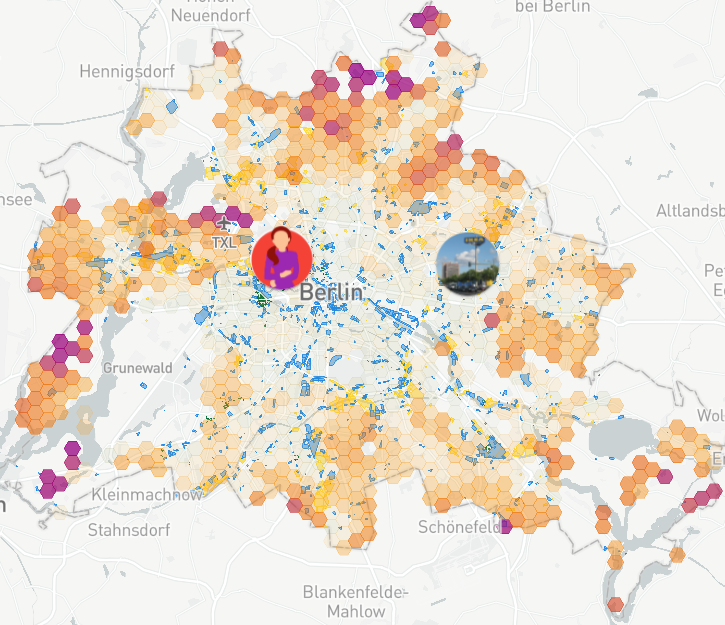
\includegraphics[width=7cm]{persona-landsberger-01}
    \end{subfigure}%
    \begin{subfigure}{.5\textwidth}
        \centering
        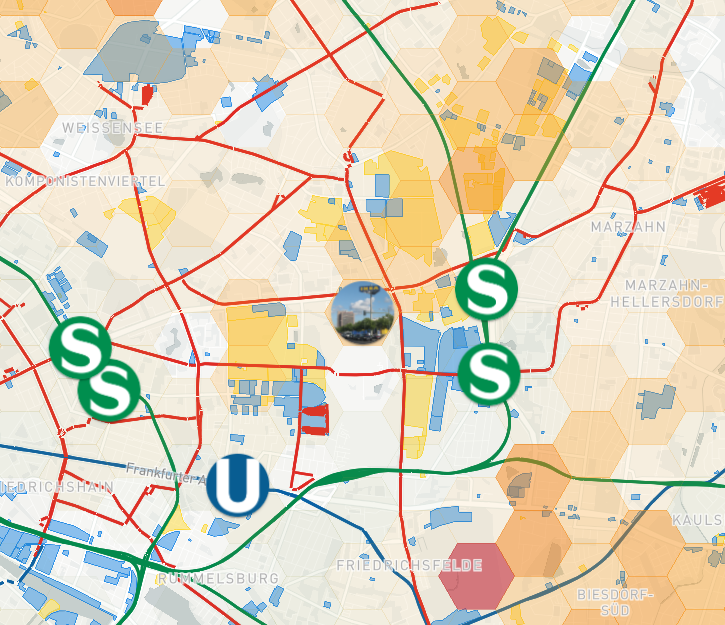
\includegraphics[width=7cm]{persona-landsberger-03}
    \end{subfigure}
    \caption{Persona Gewerbe- und Industriegebiet Landsberger Allee}
    \label{persona-landsberger-allee}
\end{figure}

Eine Anbindung an die Innenstadt bieten als weitere Verkehrsmittel des ÖPNV die U-Bahn-Station Magdalenenstraße, sowie die S-Bahn-Stationen Landsberger Allee, Storkower Straße, Springpfuhl und Pölchaustraße. Allerdings sind diese nicht fußläufig erreichbar. Insbesondere außerhalb der Stoßzeiten sind diese bedingt durch den geringeren Takt der Straßenbahn nur schwer zu erreichen.

\paragraph{Lösungsansätze}
Um die Anbindung an die anderen Verkehrsmittel des öffentlichen Nahverkehrs zu erhöhen, könnte zunächst eine Erhöhung der Taktung der Straßenbahn veranlasst werden. Zusätzlich könnte eine Nachtbuslinie eingerichtet werden, um die stark verringerte Taktung der Straßenbahn zwischen 0:00 und 07:00 Uhr zu kompensieren. Durch die Einrichtung eines Mobilitäts-Hubs (Jelbi Station) könnten beispielsweise Leihfahrräder zur Verfügung gestellt werden um die Wegzeit zur nächsten S- oder U-Bahn-Station zu verringern. Gegebenenfalls könnte ein solcher Mobilitäts-Hub auch durch die Kooperation mehrerer ortsansässiger Unternehmen realisiert werden.

\subsubsection{Der dicht besiedelte Osten Marzahn-Hellersdorfs}
\paragraph{Detailbetrachtung der Verkehrsinfrastruktur im dicht besiedelte Osten Marzahn-Hellersdorfs}
Der östliche Teil Marzahn-Hellersdorfs ist von einer sehr hohen Einwohnerdichte geprägt. Gleichzeitig existiert keine vielfältige Verkehrsinfrastruktur. Die ÖPNV-Anbindung in diesem Gebiet ist stark von der Straßenbahninfrastruktur geprägt. Die Straßenbahnhaltestellen Alte-Hellerdorfer und Michendorfer Straße bieten eine gute Anbindung innerhalb des Kiezes, Gebiete die außerhalb des Straßenbahnnetzes liegen, sind vom östlichen Rand Marzahn-Hellersdorfs jedoch kaum erreichbar. Die nächste S-Bahnstation Mehrower Allee ist mit dem Bus 30~Minuten entfernt. Der nächstgelegene U-Bahnhof Hellersdorf ist selbst mit dem Bus oder der Tram mindestens 15~Minuten entfernt.

\begin{figure}
    \centering
    \begin{subfigure}{.5\textwidth}
        \centering
        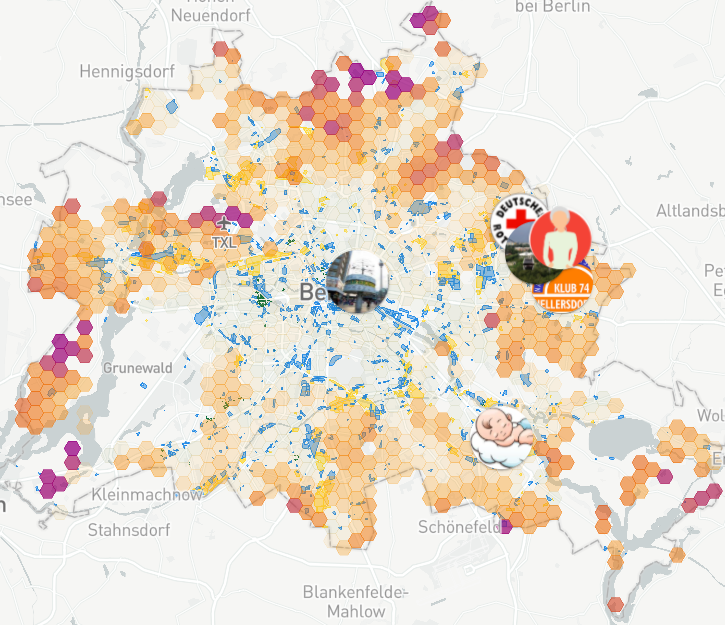
\includegraphics[width=7cm]{persona-marzahn-01}
    \end{subfigure}%
    \begin{subfigure}{.5\textwidth}
        \centering
        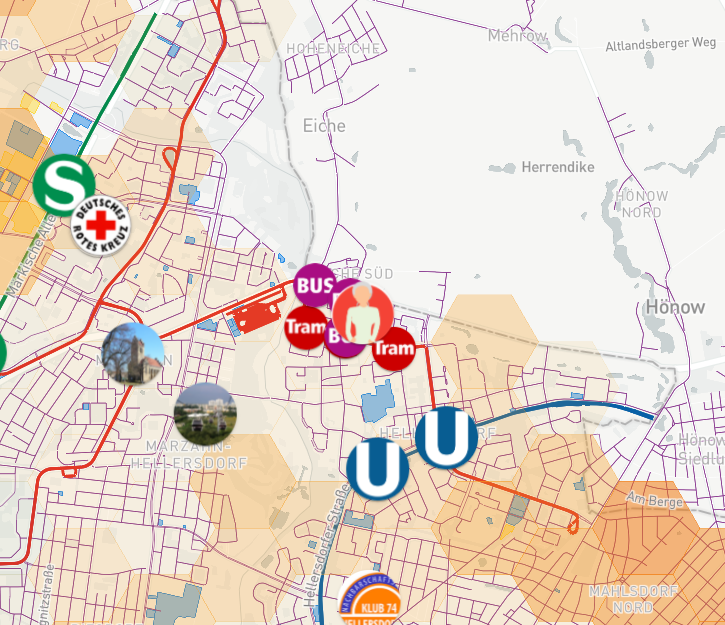
\includegraphics[width=7cm]{persona-marzahn-02}
    \end{subfigure}
    \caption{Der dicht besiedelte Osten Marzahn-Hellersdorfse}
    \label{persona-marzahn-hellersdorf}
\end{figure}

Von der aktuellen Verkehrssituation sind Arbeitnehmer*innen die in anderen Bezirken tätig sind besonders betroffen. Aber auch Senior*innen die sich innerhalb des Bezirks bewegen und beispielsweise in der Nachbarschaft engagieren, stehen vor großen Herausforderungen. Wichtige Begegnungsstätten, wie das Deutsche Rote Kreuz und der Nachbarschaftshilfe Klub~74~e.V. sind mit dem ÖPNV nicht in unter 30~Minuten erreichbar. Weitere Wege, beispielsweise bis zum Alexanderplatz, sind zwar mit der Straßenbahn erreichbar, setzen aber eine Reisezeit von mindestens 45 Minuten voraus.

\paragraph{Lösungsansätze}
Um die Erreichbarkeit innerhalb des Bezirks zu verbessern, sollte die Taktung der bestehenden Bus- und Straßenbahn Linien erhöht werden. Um die Anbindung an das übrige Stadtgebiet zu stärken, sollte die Anbindung an die S-Bahnstation Mehrower Allee und den U-Bahnhof Hellersdorf verbessert werden. Zu diesem Zweck könnten Expressbus-Linien eingerichtet werden, die die bestehende ÖPNV-Infrastruktur besser verknüpft.

\subsubsection{Gewerbegebiet Gradestraße}
\paragraph{Detailbetrachtung der Verkehrsinfrastruktur am Gewerbegebiet Gradestraße}
Anhand der genaueren Betrachtung von Gewerbedichte und Lücken innerhalb der Verkehrsinfrastruktur konnte das Gewerbegebiet an der Gradestraße, Ecke Tempelhofer Weg identifiziert werden. In diesem Gewerbegebiet im nördlichen Britz, sind international agierende Unternehmen und wichtige Arbeitgeber wie Kieback\&Peter GmbH, Linde Gas Deutschland und Terra Naturkost Handels KG angesiedelt. Zusätzlich zur hohen Industrie- und Gewerbedichte, weist das Gebiet eine verhältnismäßig hohe Einwohnerdichte auf. Die Verkehrsanbindung des Gewerbegebiets Gradestraße ist jedoch mangelhaft.

\begin{figure}
    \centering
    \begin{subfigure}{.5\textwidth}
        \centering
        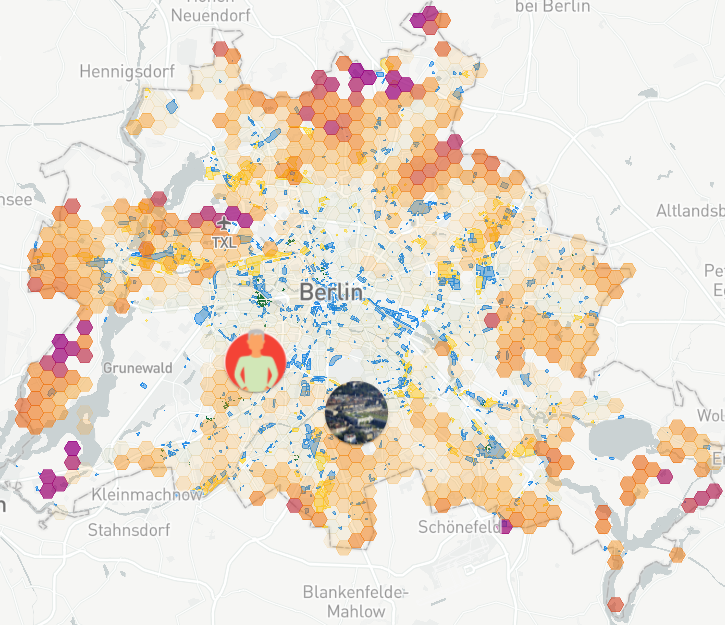
\includegraphics[width=7cm]{persona-britz-01}
    \end{subfigure}%
    \begin{subfigure}{.5\textwidth}
        \centering
        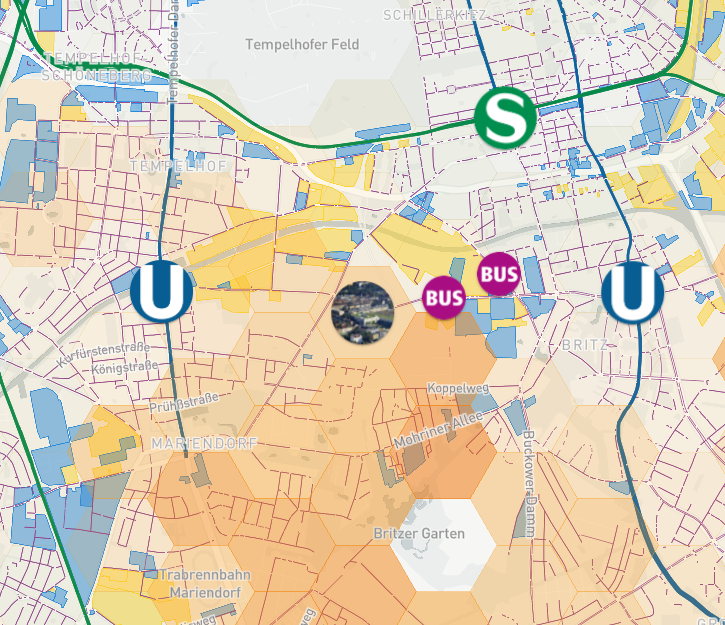
\includegraphics[width=7cm]{persona-britz-02}
    \end{subfigure}
    \caption{Gewerbegebiet Gradestraße}
    \label{persona-britz}
\end{figure}

Die Erreichbarkeit des Gewerbegebiets Gradestraße ist stark von der guten Anbindung an die Stadtautobahn abhängig. Der ÖPNV ist in der Nähe des Gewerbegebiets nur unzureichend ausgebaut. Ausgehend von dem Gewerbegebiet sind die Buslinien 170 und M44 fußläufig erreichbar. Die Buslinie 170 wird außerhalb der Stoßzeiten nur im 20~Minuten-Takt bedient und selbst die regelmäßiger verkehrende Linie M44 bietet keine ausreichende Anbindung an den ÖPNV. Die U-Bahnstationen Blaschkoallee und Ullsteinstraße sind je 26 ~ehminuten und 9~Bus-Minuten entfernt. Die nächste S-Bahnstation (Hermannstraße) ist sogar 32~Gehminuten entfernt. Selbst mit dem Bus M44 ist die S-Bahnstation Hermannstraße, aufgrund von vier Zwischenhalten 17~Minuten entfernt.

\paragraph{Lösungsansatz 1: Erhöhte Taktung und neue Buslinie}
Aktuell gibt es in Britz und dem Raum Gradestraße keine laufenden oder geplanten Infrastrukturprojekte.\footcite{NahverkehrsplanBerlin} Damit die Anbindung des Gewerbegebiets verbessert werden kann, sollte zunächst die Erreichbarkeit der bestehenden ÖPNV-Infrastruktur verbessert werden. Durch eine erhöhte Taktung des Busverkehrs außerhalb der Stoßzeiten wäre es möglich, dass im Schichtsystem tätige Arbeitnehmer*innen den ÖPNV anstelle des Individualverkehrs nutzen können. Zusätzlich könnte die Einführung einer neuen Express-Linie in Richtung der S-Bahnstation Hermannstraße die Wegzeit deutlich verkürzen. Auf diese Weise könnte die Attraktivität des ÖPNV deutlich gesteigert werden.

\paragraph{Lösungsansatz 2: Ausbau des Straßenbahnnetzes}
Im Nahverkehrsplan des Landes Berlin wird zumindest der Bedarf zum Ausbau des Straßenbahn-Netzes im Süden des Bezirks Neukölln identifiziert. Die konkrete Planung des Vorhabens steht noch aus, könnte aber tatsächlich zu einer deutlichen Verbesserung der Verkehrssituation in der Nähe des Gewerbegebiets Gradestraße beitragen.\footcite{NahverkehrsplanBerlin}
